\section{Transition to Peer-to-Peer Delivery}

A peer wishing to download a file using automated swarming first tries to download it from the origin web server using a traditional client-server download.  
If at some point one of the following conditions occurs, the client switches to peer-to-peer delivery:
\begin{enumerate}
\item First, the client waits a maximum number of seconds $T$ after the start of a download, to receive the first byte of data from the origin server.  
First data byte means any byte received from the origin--a header or content byte.  TCP connection handshake packets do not count as a data byte.
If $T$ seconds pass without the client receiving any data, it transitions to a peer-to-peer delivery.  This allows the system to decide quickly whether the origin server is over-burdened.   
\item After the client begins receiving data from the server, it monitors whether the download rate falls below a certain 
threshold of $R$ bytes per second over the last $W$ seconds.  It starts measuring this after the first byte is received\footnote{This means that it will
only ever decide that the server is slow after $W$ + the time it took to receive its first data byte, or at least $W$, and at most $T$ + $W$.}.  
If the receive rate ever drops below $R$, the client transitions to peer-to-peer delivery.  
This is to accomodate servers with slow connections or servers that become overloaded during a download.
\end{enumerate}

\section{Finding Peers}

Peers interested in downloading the same file find each other using a Distributed Hash Table (DHT).
A DHT is essentially a distributed P2P hash table that maps a key to a value.  A client can,
for example, query the DHT with a key of ``file x block y" and get a list of peers with block y
of file x.

We run a DHT using the Bamboo OpenDHT code on approximately 1000 PlanetLab peers\footnote{Typically about 300 are stably active.}.  
3 peers are designated as ``gateways" that the others contact to bootstrap themselves into the DHT.  After servers join the DHT, each 
creates a web service that accepts queries from peers outside the DHT.  When a server receives a
query, it forwards it through the DHT, retrieves the answer, and returns the answer to the requestor. 
Members of the DHT run continously, servicing requests.
Data is stored as key, value maps, with many values storable per key.  
If there are more than ten values stored, only the first 10 values are returned for the first request. 
If a peer wants more than the first 10 values, it must make a repeat query and request values 11-20, etc.  
We use the DHT to store peer information, to help peers find each other.  Anf alternative design would be to store blocks of the file in the DHT.  
However, this would put more stress on the DHT, due to bandwidth demands.  This design would also violate design goal \#4.

In order for our clients to use this DHT, each is given a list of all known DHT members out-of-band.  When they are instructed to download a file, 
they ``port sniff" on the web service ports of DHT members, to create a list of live DHT members.  
They query 10 DHT servers at a time, until they have found at least 5 that are active.
They then round robin across the list of known active members for queries they later perform.

When a peer performs a query, for example for a key ``http://host/filename peers for block num y'', it requests this key and also a ``redundant key" for the same, 
like ``http://host/filename peers for block num y key redundancy 1''\footnote{Note that Bamboo actually queries a hash of the query string, not the full string.}.  
It requests both keys from 2 different gateways (using the round robin described above), 
thus the total number of queries per request is 4.  
The reason for this is that sometimes keys are hosted on poorly connected members of the DHT, making response time slow.
Sometimes gateways themselves are temporarily slow, so using multiple gateways per request avoids this slowdown, as recommended by the authors of OpenDHT \cite{opendht_embarrassing}.
The client times out DHT requests after 60 seconds if no response is received, as a reasonable value to keep from 
overloading the DHT.  When a request times out, the client will automatically retry it, for up to 3 times, before giving up on the request.

When a client transitions to peer-to-peer delivery, it first checks to see if it knows enough meta-data about the file it is downloading.  
It needs to know the size in order to look up peer lists.
If the client has previously received a TCP header with size information from the origin, it has the information it needs.  If it doesn't, it
queries the DHT, using a key of the URL being downloaded, for known meta-data.  
Other peers store the meta-data here when they have previously downloaded the file (Fig.~\ref{fig:yanc_step_1}). 
While performing this meta-data lookup, a client also does an HTTP HEAD request for the file to the origin server, 
and uses the first successful response from either of these two to determine file size.  
If there is no meta-data listed in the DHT, a client continues to poll the DHT every 5 seconds to see if meta-data for the file has appeared.  At some point
either the meta-data will appear in the DHT or the HTTP HEAD request will return (with size information) and the peer will then have the meta-data 
it needs and will start  peer-to-peer delivery.

\section{Peer-to-Peer Delivery}

To accomplish peer-to-peer delivery, the client randomly chooses $b$ blocks of the file to download at a time (Fig.~\ref{fig:yanc_step_2}).  
It retrieves the list of peers who have each block by querying the DHT for a key composed of
the URL concatenated with a given block number (like ``http://host/filename\_peers\_for\_block\_num\_y").  
If there are no peers listed yet for that block, it polls the DHT every 1 second to see if new peers have arrived.
While it does not yet have a list of any peers, it also contacts the origin and starts a download of the block, so as to 
not waste time in the case that no peers are ever available.  This is useful for some peers that have DHT connections that are too slow.
When it receives a peer list from the DHT, the client shuffles the list randomly, then connects to each peer one at a time, and requests the block.  
If the peer begins to serve the block, the client closes its connections to the origin, if open, and downloads the rest of the block from that peer.  
If the peer interrupts the connection or is not online, the client chooses the next peer until it runs out of peers to use.  
Then it repeats the steps for that block, but requesting the next 10 peers listed in the DHT.

When a peer only has a few blocks remaining, it tries to download the last few blocks from several peers (redundantly), in an effort to avoid the last block problem \cite{last_block}.  
It downloads all remaining blocks from a total of $b$ peers, so if $b$ is set to 6 and 3 blocks are left, it downloads each remaining block from 2 redundant peers, with the
last block being downloaded from all 6 peers redundantly.

\section{Sharing}

Clients must share information using the DHT to make automatic swarming work.  First, when a peer learns the size of the file 
from its original HTTP request or its later HTTP HEAD request, it stores this ``meta-data" about the file
in the DHT.  It does this by querying to see if this data has already been stored there.  If it hasn't, it stores it by setting the value of the URL in the DHT to the file's size. 
Later peers then use this to retrieve the meta-data for the file if necessary.
Second, whenever a client downloads a block, it adds itself to the list of peers willing to share that block (Fig. \ref{fig:yanc_step_3}). 
Finally, after completing a file download, the client lingers a certain number of seconds.  After its linger time is up, it drops all current connections to peers 
and performs DHT remove requests to remove itself from the peer lists in the DHT.

\begin{figure*}
  \begin{center}
    \subfigure[Peer downloads meta-data]{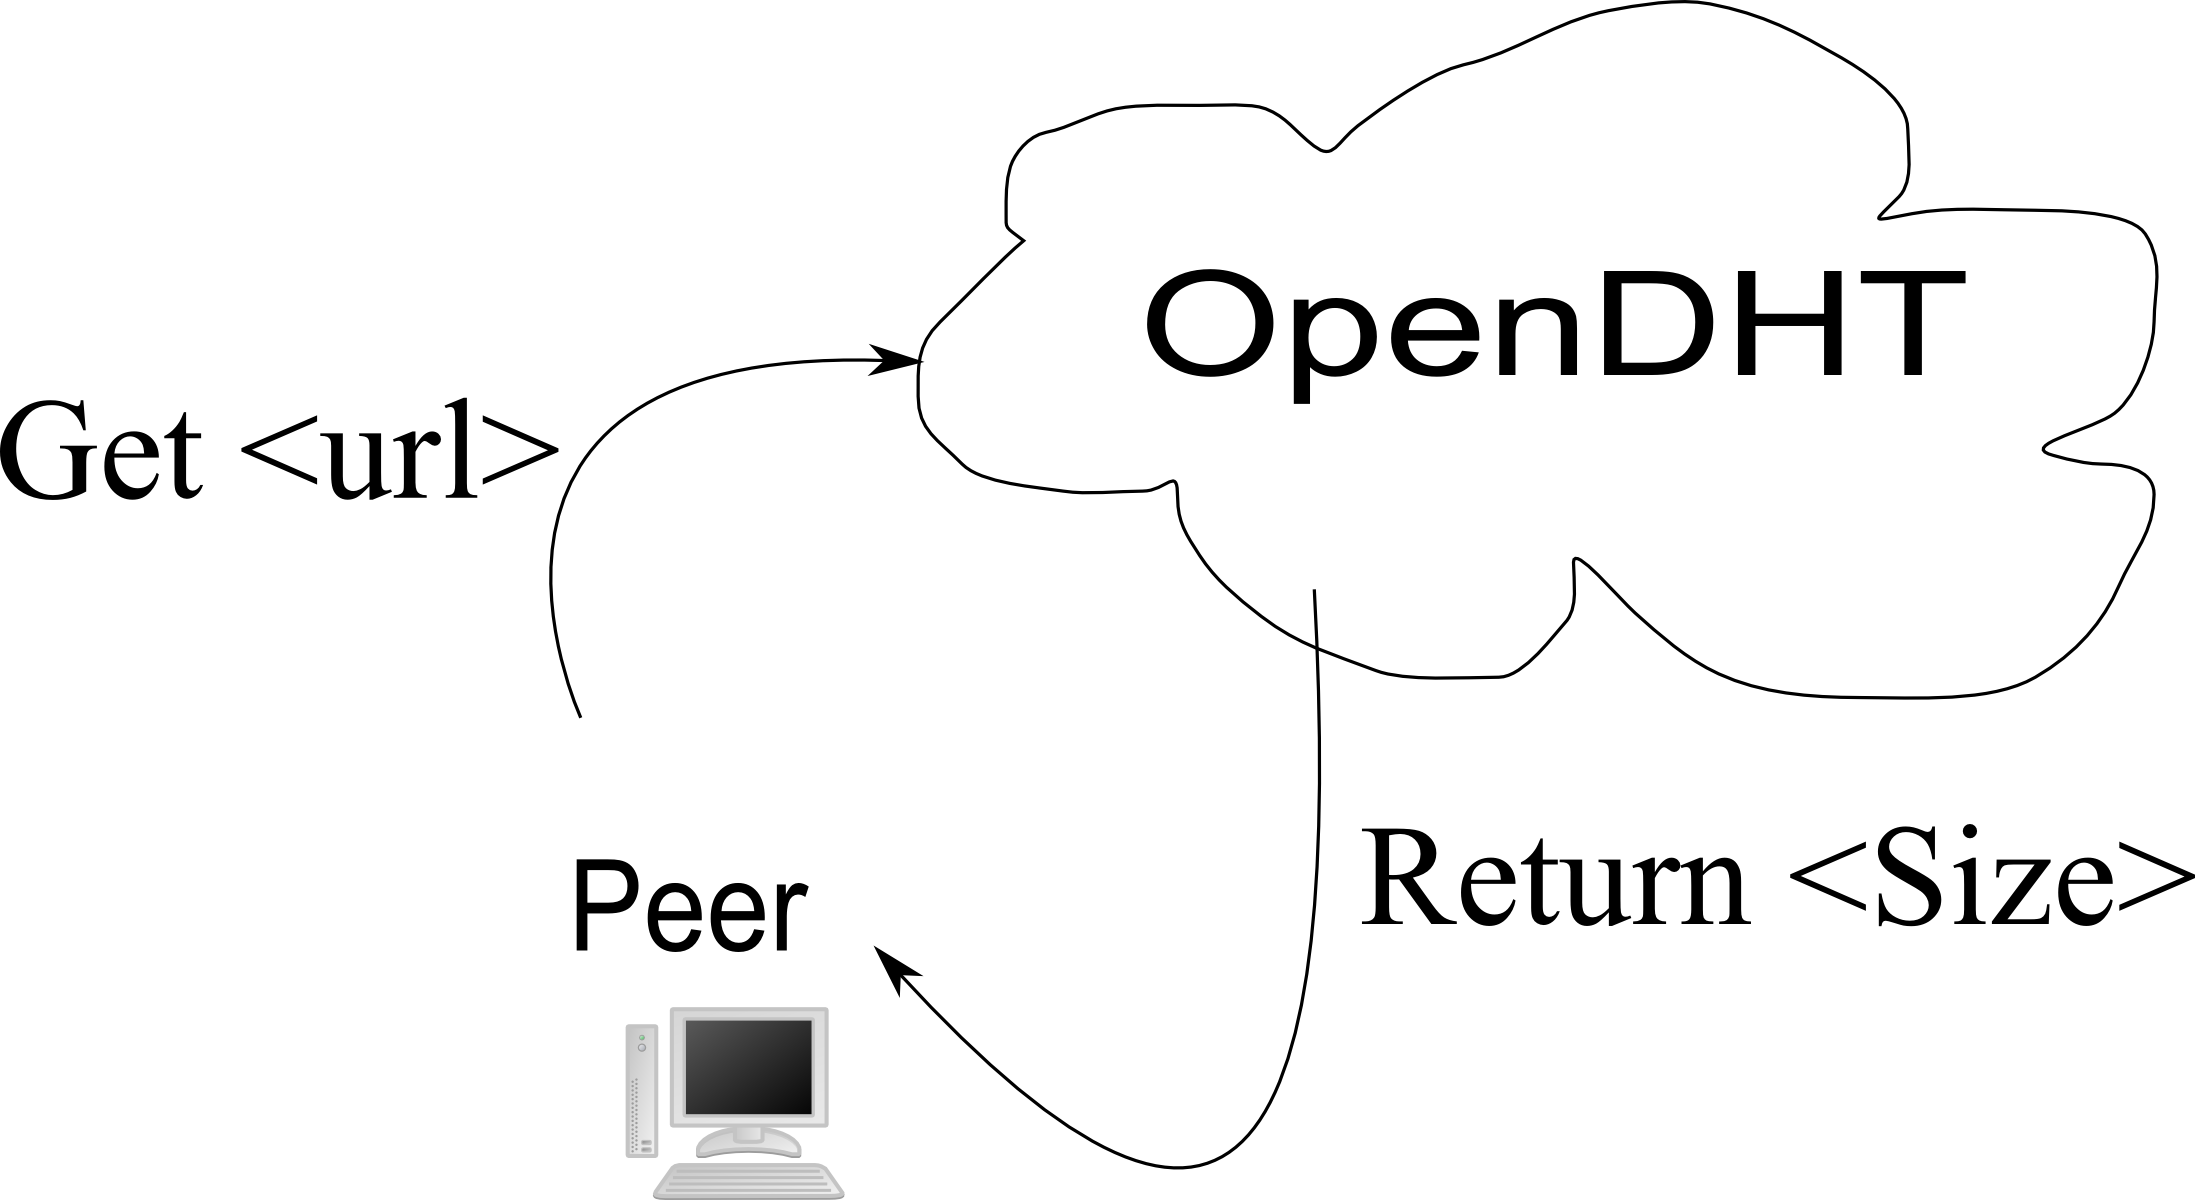
\includegraphics[width=7cm]{description_pics/peer_step_1.png}\label{fig:yanc_step_1}}
    \subfigure[Peer downloads a list of peers that have a block]{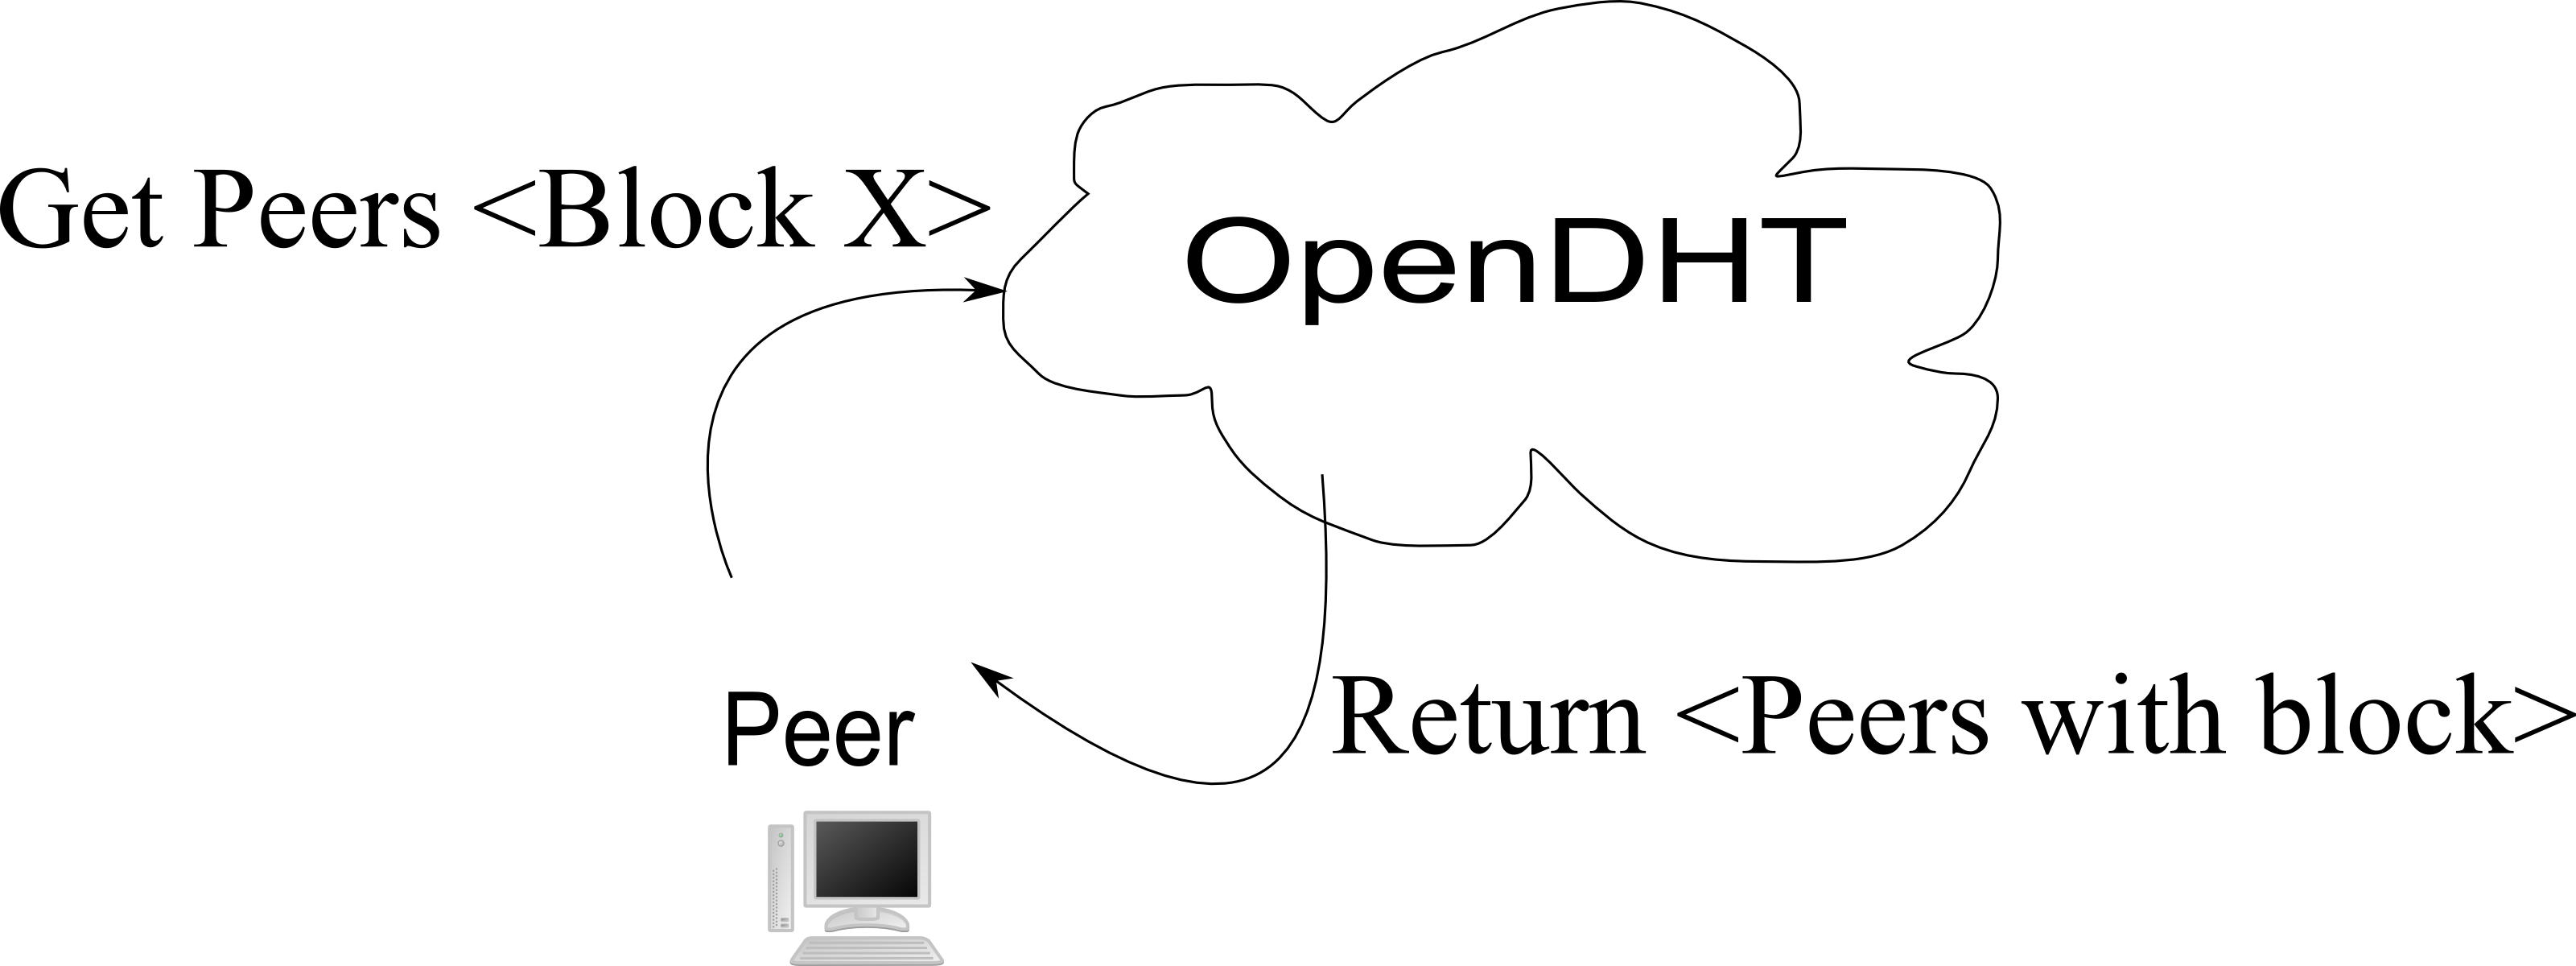
\includegraphics[width=10cm]{description_pics/peer_step_2.png}\label{fig:yanc_step_2}}
    \subfigure[Peer adds itself to list of peers who have the block]{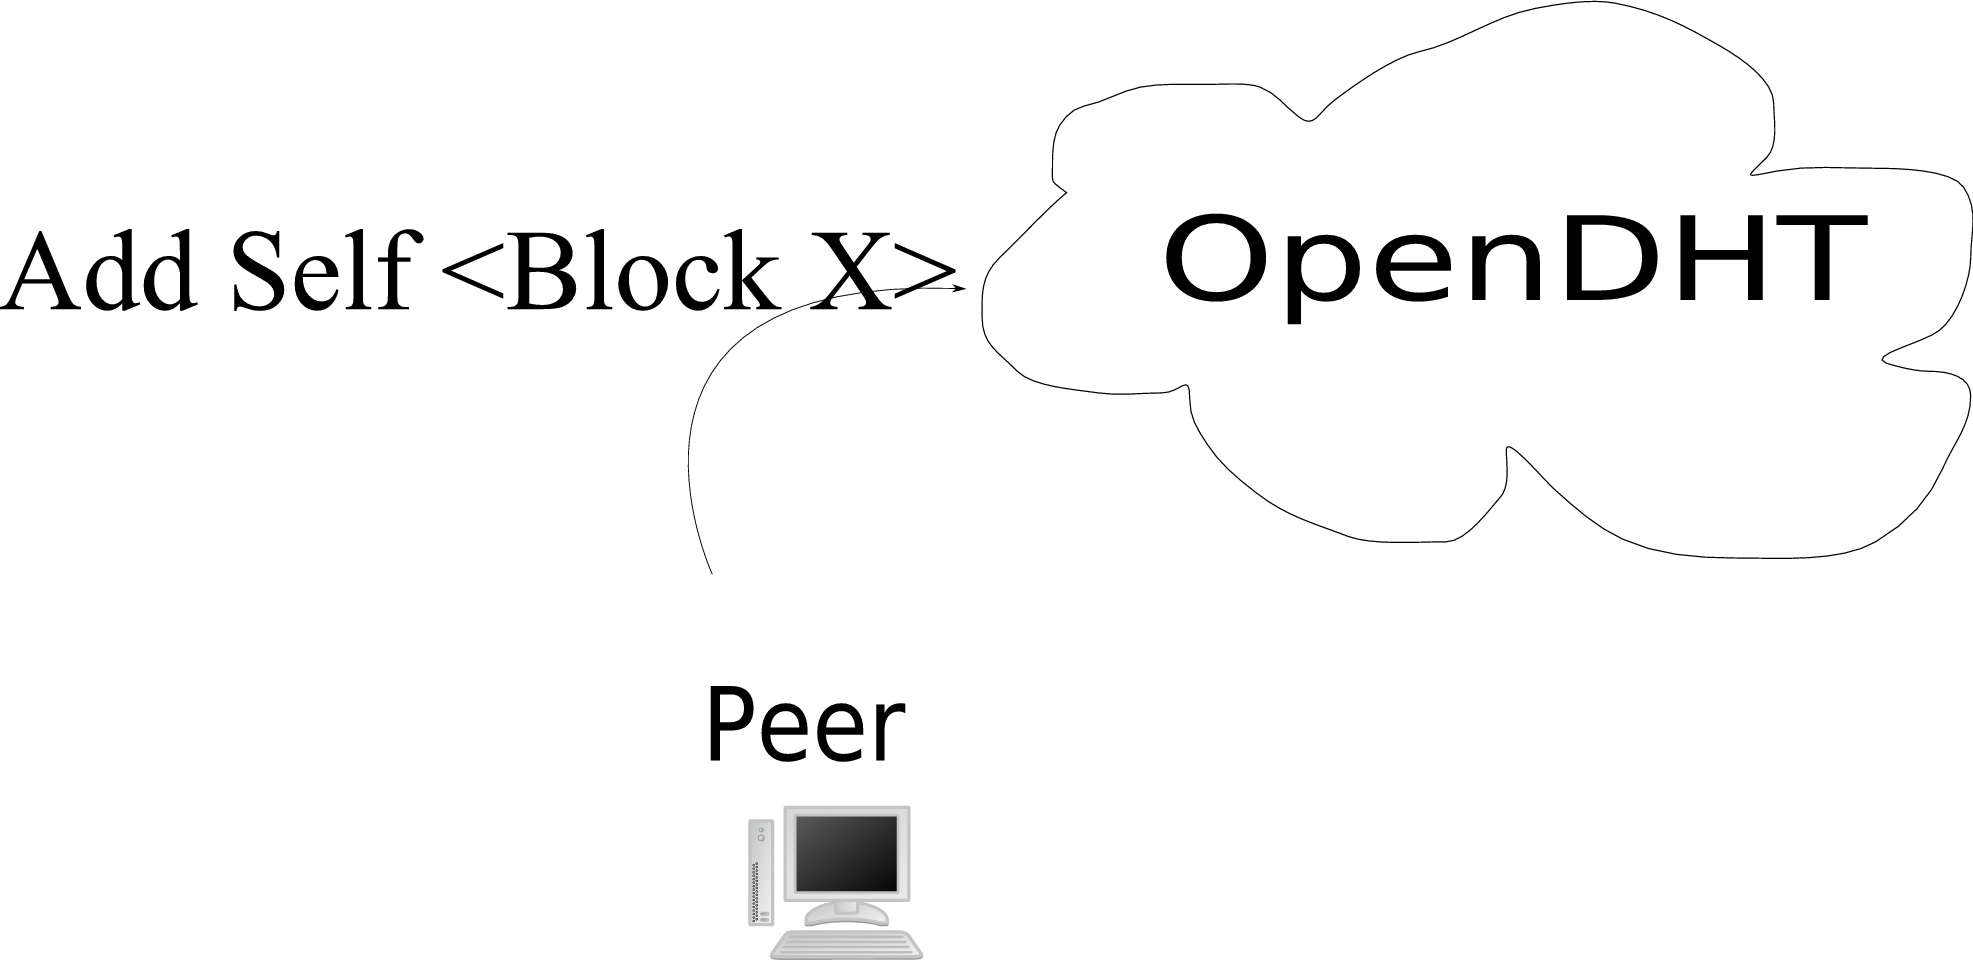
\includegraphics[width=8cm]{description_pics/peer_step_3.png}\label{fig:yanc_step_3}}
    \caption{Steps to accomplish a peer-to-peer-web download}
    \label{fig:yanc_all_steps}
  \end{center}
\end{figure*}